\documentclass[12pt]{article}

\usepackage[tables,figures,master]{updiplom}
\usepackage[utf8]{inputenc}
\usepackage{amsmath}
\usepackage{amsthm}
\usepackage{booktabs}
\usepackage{algorithm}
\usepackage{algpseudocode}



%%% Obecné věci
\newcommand{\name}{CHANDLER}
\newcommand{\code}[1]{\texttt{#1}}
\newcommand{\sep}{\,|\,}
\newcommand{\docs}{\mathbb{D}}
\newcommand{\yes}{$\times$}
\newcommand{\fyes}{\fbox{$\times$}}
\newcommand{\foreach}{\mbox{pro všechna }}
\newcommand{\pravekdyz}{\mbox{právě když }}

%%% Nadpisy
\newcommand{\ssection}[1]{\subsection{#1}}
\newcommand{\sssection}[1]{\subsubsection{#1}}

%%% Závorky
\newcommand{\addk}[1]{\left(#1\right)}
\newcommand{\addh}[1]{\left[#1\right]}
\newcommand{\adds}[1]{\left\{#1\right\}}
\newcommand{\addsp}[1]{\left<#1\right>}

\newcommand{\strong}[1]{{\em #1}}

%%% Logické spojky
\newcommand{\logand}{\,\wedge\,}
\newcommand{\logor}{\,\vee\,}
\newcommand{\eq}{\Leftrightarrow}
\renewcommand{\implies}{\Rightarrow}

%%% Používané funkce
\DeclareMathOperator{\tfidf}{tf-idf}
\DeclareMathOperator{\stem}{stem}
\DeclareMathOperator{\score}{sc}
\DeclareMathOperator{\wcount}{sf}
\DeclareMathOperator{\getdocs}{R}
\DeclareMathOperator{\AND}{AND}
\DeclareMathOperator{\OR}{OR}
\DeclareMathOperator{\NOT}{NOT}
\DeclareMathOperator{\rank}{rank}
\newcommand{\invstem}{\stem^{-1}}
\newcommand{\alldoc}{\mathbb{D}}

%%% FCA věci
\newcommand{\context}{\addsp{X, Y, I}}
\newcommand{\lattice}{\mathcal{B}(X, Y, I)}
\newcommand{\AB}{\addsp{A, B}}
\newcommand{\up}{^{\uparrow}}
\newcommand{\down}{^{\downarrow}}
\newcommand{\updown}{^{\uparrow\downarrow}}
\newcommand{\downup}{^{\downarrow\uparrow}}


\newtheorem{mydef}{Definice}





\title{Vyhledávač založený na formální konceptuální analýze}
\author{Lukáš Havrlant}
\year{2011}
%\date{21. květen 2009}

\docinfo{Lukáš Havrlant}{Vyhledávač založený na formální konceptuální analýze}

\annotation{Napovídáním souvisejících dotazů může vyhledávač pomoci uživateli rychleji najít dokumenty, které potřebuje. V práci se zabývám tvorbou vyhledávače s webovým rozhraním, který pracuje nad uzavřenou sadou dokumentů. Po položení dotazu dokáže napovědět konkrétnější, obecnější a podobný dotaz, což je realizováno pomocí formální konceptuální analýzy.}

\thanks{Děkuji Mgr. Janu Outratovi, Ph.D. za vedení této diplomové práce a za rady při konzultacích.}

\begin{document}

\maketitle
\newpage


%%% Text diplomové práce.
\section*{Úvod}
\addcontentsline{toc}{section}{Úvod}

Současné vyhledávače si uchovávají obsah, nad kterým mají vyhledávat, ve formě indexu, což je struktura v principu podobná indexu v knize. Uživateli stačí vložit do vyhledávacího pole svůj dotaz a vyhledávač z indexu získá potřebná data a zobrazí uživateli výsledek, obvykle ve formě nějakého uspořádaného seznamu odkazů na dokumenty. Pokud není uživatel spokojený s výsledky, musí přeformulovat svůj dotaz tak, aby lépe vystihoval to, co chce najít. 

Tento problém je typický pro slova, která mají několik významů. Například pokud ve webovém vyhledávači vyhledáme slovo \uv{jaguár}, tak vyhledávač nemůže vědět, zda chceme hledat auto, zvíře nebo ještě něco jiného. Pokud má přístup k historii hledání daného uživatele, může pomocí ní přizpůsobit výsledky. Ale může také uživateli zobrazit návrhy na nový dotaz, například \uv{jaguár auto} nebo \uv{jaguár zvíře}, po jejichž vyhledání se výsledky velmi zpřesní. 

Otázkou je, jak tyto návrhy získat. Pokud si vyhledávač uchovává historii všech hledání, která uživatelé provádějí, může se je pokusit vytáhnout právě z této historie. Pokud ovšem tato data vyhledávač nemá, nebo jich má málo, musí se použít jiná metoda. 

Tato práce popisuje metodu, jak získat podobné dotazy pomocí formální konceptuální analýzy (anglicky Formal concept analysis, dále jen FCA) pouze na základně znalosti obsahu dokumentů. FCA pracuje s tabulkovými daty, ve kterých hledá nějaké potenciálně zajímavé shluky dat. Tyto shluky pro nás budou představovat množiny dokumentů, které jsou nějakým způsobem podobné a které sdílí nějaká zásadní klíčová slova. Tato klíčová slova poté dále využijeme při genrování návrhů na nové dotazy. 

Diplomová práce je rozdělena do několika kapitol. V první kapitole, \uv{Information retrieval}, je popsáno, jakým způsobem pracuje samotné jádro vyhledávače. 

\newpage
\section{Information retrieval}

Tato sekce se zabývá budováním samotného vyhledávače, jehož výsledky budou zobrazeny uživateli a také budou použity jako vstup do formální konceptuální analýzy. 

Cílem je popsat tvorbu vyhledávače, který bude umět stáhnout z webu požadované dokumenty, zaindexovat je a následně v nich vyhledávat. Dokumenty mohou být buď obyčejné webové stránky nebo složitější soubory, například PDF. 

\subsection{Jak funguje vyhledávač}
V této části si popíšeme, jak může obecný vyhledávač fungovat. 

\subsubsection{Pojmy související s vyhledávačem}
\begin{description}
\item[Sada dokumentů] Na začátku máme nějakou sadu dokumentů, nad kterými chceme vyhledávat. Tato sada může být libovolná -- může se jednat o webové stránky, o lokální dokumenty na osobním počítači nebo o emaily na serveru. V případě webových vyhledávačů typu Google je pak sadou dokumentů \uv{všechno, co lze nalézt na webu}, v případě vyhledávačů v moderních operačních systémech je sadou \uv{všechno, co lze nalézt na počítači}. 

Sada dokumentů může být buď statická, nebo dynamická. Statická sada je taková sada, která se nemění buď nikdy nebo málokdy. Může to být například vyhledávač PSČ. Dynamická sada se naopak mění poměrně často, například webové stránky. Velké vyhledávače častěji pracují s dynamickou sadou dokumentů. 

\item[Uživatel] Uživatel je obecné označení toho, kdo pracuje s vyhledávačem. Typicky se jedná o nějakého člověka, ale může to být i program, který například každý den kontroluje počet dokumentů na dané klíčové slovo a při zvýšení pošle někomu informační email. 

\item[Dotaz] Pomocí dotazů komunikuje uživatel s vyhledávačem. Dotaz je nějaký seznam slov, který reprezentuje to, co uživatel chce najít. Může se jednat o jednoduché dotazy typu \uv{auto}, ale také o složitější otázky jako \uv{Jaký je smysl života?} Slovům v dotazu říkáme klíčová slova. 

Vyhledávač může uživatelům umožnit používat v dotazu různé operátory, kterými může uživatel zpřesnit svůj dotaz. Typické operátory jsou logické operátory AND, OR a NOT. Webové vyhledávače umožňují například vyhledávat na určité doméně pomocí SITE operátoru, vyhledat odkazující stránky pomocí LINK operátoru a podobně. 

\item[Výsledky vyhledávání] Po položení dotazu zobrazí vyhledávač výsledky. Obecně se jedná o nějaké zkrácené zobrazení dokumentů, které vyhovují danému dotazu. Typicky jde o seznam odkazů na dané dokumenty, ale v některých případech může vyhledávač přímo zodpovědět položenou otázku. Například na otázku o smyslu života může odpověď 42. 

Samotný seznam dokumentů bývá obvykle seřazen podle nějakých kritérií. Těchto kritérií bývá poměrně hodně a vyvážit je tak, aby vyhledávač vracel co možná nejlepší výsledky je obtížný úkol, kterým se tato diplomová práce nebude více zabývat. 

Mezi výsledky může být kromě seznamu odkazů i nějaká další informace. Současné webové vyhledávače například umí opravovat překlepy, přehrát video odpovídající klíčovým slovům, vypočítat jednoduché matematické operace nebo napovědět dotaz, který by vedl k přesnějším výsledkům. 
\end{description}


Dále si představíme dva modely, jak může vyhledávač fungovat. Naivní model a model používající index.

\subsubsection{Naivní model vyhledávače}

Naivní model vyhledávače funguje tak, že po položení dotazu začne vyhledávač procházet všechny dokumenty a kontroluje, jestli některý z dokumentů odpovídá dotazu. Pokud ano, vrátí tento dokument mezi výsledky. 

Tento model je velice jednoduchý, ale není příliš efektivní. V současné době můžeme mít sady dokumentů, které obsahují miliony či miliardy položek, takže chceme-li znát výsledky řádově za desetiny sekund, není možné je při každém dotazu všechny procházet.

\subsubsection{Vyhledávač používající index}
Mnohem efektivnější je použít index. Jedná se o podobnou strukturu, kterou můžeme najít v některých, obzvlášťě odborných, knihách. Protože v klasické tištěné knize nemůžeme nijak \uv{vyhledávat}, dává se na konec knihy seznam nejdůležitějších slov, která kniha obsahuje, spolu s čísly stránek, na kterých se pojem vyskytuje. Takže chce-li uživatel nalézt stránky obsahující slovo \uv{derivace}, podívá se do indexu, kde hned zjistí, že slovo se vyskytuje na té a té stránce. 

Podobný princip můžeme použít i ve vyhledávačích. Nebudeme ale vytvářet index z důležitých slov, ale ze všech slov, která se v dokumentech vyskytují. Vytvoříme tak slovníkovou strukturu, kde klíčem bude slovo a hodnotou bude seznam dokumentů, které dané slovo obsahují. Při položení dotazu pak může vyhledávač rychle zjistit jaké dokumenty obsahují dané klíčové slovo prostým nahlédnutím do tohoto slovníku. 

Spolu s tím si můžeme uložit informace i o tom, kolik daných slov daný dokument obsahuje, což můžeme dále využít při řazení dokumentů. 

Celou práci vyhledávače tak můžeme rozdělit do dvou částí -- budování a upravování indexu a hledání odpovědí na dotaz. Zde je nutné dát pozor na to, jak velká je sada dokumentů a zda je statická nebo dynamická. Samotné budování indexu můžeme ještě rozdělit na dvě podčásti: předzpracování dokumentů a technická realizace indexu. 

\subsection{Vyhledávač \name}

Součástí této diplomové práce je naprogramovaný vyhledávač \name, který bude v dalších částech textu popsán. \name{} je vyhledávač napsaný v Pythonu 3. Pracuje se statickou sadou dokumentů, předpokládá se, že se sada dokumentů bude měnit pouze nárazově jednou za čas. Samotná sada dokumentů, nad kterou má vyhledávač pracovat, nebude příliš velká, řádově stovky dokumentů. 

Jedná se vyhledávač používající index. Při budování indexu je vstupem seznam URL adres, které si vyhledávač sám stáhne a zaindexuje je. Výsledný index je pak uložen do několika souborů, ke kterým pak vyhledávač přistupuje. 

\name{} má rozumět logickým operátorům AND, OR a NOT. Po zadání dotazu má vrátit výsledky seřazené podle relevance, kterou spočítá pomocí klasického tf–idf algoritmu. Výstup bude textový ve formátu JSON, se kterým pak mohou pracovat další programy, v tomto případě webové rozhraní, které je napsáno v PHP. 

Další částí vyhledávače je hledání souvisejících dotazů. Tato část bude podrobně rozebrána v další kapitole. V této kapitole je dále popsáno, jak \name{} buduje index a jak vrací výsledky. 

%Dále seznam dotazů, které konkretizují zadaný dotaz, tj. seznam nových klíčových slov, které můžeme přidat k současnému dotazu, abychom získali přesnější výsledky. To je případ, kdy po vyhledání \uv{jaguár} vyhledávač napoví \uv{jaguár auto}. Dále seznam podobných dotazů, což jsou dotazy, které mění jedno nebo více klíčových slov v dotazu. To je případ, kdy vyhledávač k \uv{jaguár auto} napoví \uv{jaguár zvíře}. Nakonec vyhledávač zobrazí i obecnější dotaz. K dotazu \uv{jaguár zvíře} tak může zobrazit \uv{jaguár}.  


\subsection{Předzpracování dokumentů}
\label{prepr}
Při budování indexu máme na vstupu sadu dokumentů a na výstupu strukturu, která reprezentuje index této sady. Během samotného budování indexu procházíme jednotlivé dokumenty a upravujeme je do takové podoby, která se hodí pro uložení. Budeme uvažovat pouze textové dokumenty jako je HTML nebo PDF a budeme předpokládat statickou sadu dokumentů, takže se nebudeme příliš zatěžovat aktualizací indexu. 

Na samotném začátku tak musíme upravit jednotlivé textové dokumenty do nějaké kanonické podoby. To budeme dělat postupnými úpravami jednotlivých dokumentů. S každým dokumentem budeme provádět identické oprace v identickém pořadí. Jednotlivé operace budou popsány v takovém pořadí, v jakém se aplikují ve vyhledávači. 

\begin{description}
% \item[Zjištění názvu dokumentu] U některých typů dokumentů můžeme z jejich obsahu zjistit název dokumentu. Například pokud máme na vstupu HTML stránku, můžeme zjistit název stránky z TITLE elementu. U ostatních dokumentů vezmeme jako název obyčejný název souboru. Pokud zpracováváme soubor \code{prikazy.pdf}, bude názvem právě \uv{prikazy.pdf}.

\item[Odstranění formátovacích prvků dokumentu] Vstupem do algoritmu budování indexu může být soubor, který kromě samotného textu obsahuje i různé formátovací a jiné prvky. Tyto prvky pro další zpracování nepotřebujeme, takže je všechny odstraníme. Jedná se například o HTML nebo XML značky. Po aplikaci tohoto bodu už bychom měli mít pouze čistý text. 

\item[Ponechání písmen] Text obsahuje spousty různých znaků, které jsou vyhledávači téměř k ničemu. Jedná se o interpunkci, která typicky doplňuje text, ale při samotném vyhledávání se bez ní obejdeme. Odstraníme tak všechny znaky, které nejsou písmeny. 

Při tomto odstraňování můžeme narazit na určité problémy a může zde dojít k první ztrátě informace. Například pokud ze slova \uv{chcete-li} odstraníme spojovník, můžeme dostat buď slovo \uv{chceteli} nebo dvě slova \uv{chcete} a \uv{li}. 

\item[Odstranění bílých znaků] Pod bílé znaky spadají mezery, tabulátory a nové řádky. To jsou opět informace, které jsou zbytné a které můžeme odstranit. Namísto libovolně dlouhé posloupnosti bílých znaků tak vždy vložíme právě jednu mezeru. Tím dosáhneme toho, že všechna slova v celém dokumentu budou v jednom řádku a budou oddělena právě jednou mezerou. 

\item[Převod na malá písmena] Velikost písmen má pouze minimální vliv na hodnocení dokumentů, takže můžeme všechna písmena převést na jednotný tvar. V tomto případě na malá písmena. Můžeme sice nalézt případy, kdy ztratíme jistý kousek informace, například \uv{Prokop Buben} vs. \uv{prokop buben}), ale tento kousek je natolik zanedbatelný, že si to můžeme dovolit. 

% \item[Převod do pole] V tuto chvíli už máme text v takové podobě, že ho můžeme převézt do jiné datové struktury, a sice pole. Jako oddělovač zvolíme mezeru. Tím získáme pole, které v každé buňce obsahuje právě jedno slovo. 

\item[Odstranění stop slov] Stop slova jsou slova, která se vyskytují téměř v každém dokumentu, jsou příliš obecná a nicneříkající a tak nemá příliš velký smysl je indexovat. Typicky se jedná o předložky jako \uv{ke}, \uv{u}, \uv{na} a podobně. Pokud je odstraníme, neztratíme příliš mnoho informací, ale můžeme tím i poměrně výrazně zredukovat velikost výsledného indexu. Obecně můžeme odstranit všechna slova délky jedna nebo dva bez větší ztráty informace. 

\item[Převod na stemy] Jedna z nejdůležitějších části vyhledávače je převod slov na stemy. Stem je kořen, základ slova. Smyslem je, abychom si v indexu neuchovávali všechny tvary každého slova, ale abychom si od každé slova uchovávali ideálně jen jeden, základní tvar -- místo \uv{strom}, \uv{stromy}, \uv{stromu} tak budeme mít pouze jeden tvar \uv{strom}.

Důvody pro to máme v zásadě dva: opět se velmi výrazně sníží velikost indexu, protože namísto například pěti tvarů, budeme mít uchovaný pouze jeden tvar. Druhým důvodem je, že pokud uživatel hledá slovo \uv{strom}, pravděpodobně bude spokojený i s dokumentem, který obsahuje slova \uv{stromy} a \uv{stromu}, ale neobsahuje samotné slovo \uv{strom}. 

Algoritmus, který by k libovolnému slovu vrátil jeho základ, je poměrně komplikovaný a většinou ani není, alespoň v případě českého jazyka, příliš úspěšný. Přesto se stále vyplatí nějaký stemmer použít a ve vyhledávači použit je. 

\item[Odstranění diakritiky] Po převodu na stemy můžeme odstranit diakritiku. Odstraněním diakritiky může vzniknout několik konfliktů, které před ostraněním neexistovaly, ale je to jednoduchý způsob, jak umožnit vyhledávat i lidem, kteří diakritiku vůbec nepoužívají. Navíc ani autor nějakého dokumentu diakritiku nemusel používat a z některých dokumentů se kvůli problémům s kódováním ani písmena s diakritikou nepodaří získat. Odstraňovat veškerou diakritiku je tak nejmenší zlo. 
\end{description} 

\subsection{Uložení indexu}
V tuto chvíli máme vstupní dokumenty převedeny do tvaru, se kterým můžeme pracovat dále a můžeme vytvořit základní index. Do něj si uložíme informace o tom, ve kterých dokumentech se vyskytuje daný stem. Pokud pak budeme chtít získat dokumentu, které obsahují stem \uv{strom}, vyhledáme si v indexu záznam o stemu \uv{strom} a okamžitě získáme množinu dokumentů, která stem obsahuje. 

Bude se nám také hodit informace o počtu stemů v daném dokumentu. To využijeme během řazení dokumentů od nejvíce relevantních. Nakonec si můžeme ještě uložit informaci o počtu výskytů daného stemu ve všech dokumentech. Všechny tyto informace můžeme uložit do struktury, která vypadá takto: 

\begin{verbatim}
stem => (počet výskytů slova ve všech dokumentech, 
         [(doc1, počet výskytů v doc1), 
          (doc2, počet výskytů v doc2), 
          ..., 
          (docN, počet výskytů v docN)])
\end{verbatim}

Proměnné \code{doc1}, \code{doc2}, \dots představují ID dokumentů, které obsahují daný stem a každé slovo tak může obsahovat různou sadu docID. Pokud dokument \code{docA} stem neobsahuje, pak ve struktuře vůbec řádek \code{(docA, počet výskytů v docA)} není. 

\subsection{Vyhledání atributů dokumentu} 

V druhé části vyhledávače, která se zabývá nalezením souvisejících dotazů, budeme potřebovat znát množinu slov, která nejvíce charakterizuje daný dokument. Těmto slovům budeme říkat \uv{atributy dokumentu}. 

\subsubsection{Jak by měly atributy vypadat}

Atributy jsou poměrně běžnou součástí různých vědeckých článků, kde je ale obvykle vyplňuje sám autor pod názvem \uv{klíčová slova}. V případě vyhledávače stojíme před problémem, jak získat atributy z libovolného dokumentu nějakým obecným způsobem. 

Jednoduchým způsobem je seřazení všech stemů v daném dokumentu podle jejich četnosti od nejvíce častého. Za atributy pak můžeme vzít ty stemy, které překročí nějakou absolutní hranici (\uv{alespoň 10 výskytů v dokumentu}) nebo nějakou relativní hranici (\uv{poměr počtu daného stemu ku počtu všech stemů v dokumentu je větší než 0,05}). 

Tento postup může být úspěšný v případě, že máme pouze jeden dokument. Pokud ale máme sadu dokumentů, můžeme ještě zjistit vztah s dalšími dokumenty. Klíčové slovo pro daný dokument by totiž mělo být takové slovo, které je mezi ostatními dokumenty co možná nejvíce unikátní. 

Pokud máme sadu dokumentů, která se zabývá analýzou dat, je možné, že by v každém dokumentu bylo nejčastější slovo právě \uv{analýza}. Tím bychom dostali pro každý dokument stejné klíčové slovo a to není to, co bychom chtěli. 

Tento problém vyřešíme tím, že při hledání klíčových slov pro dokument vezmeme v potaz i to, jak často se daná slova vyskytují v ostatních dokumentech. Budeme tak hledat taková slova, která se v daném dokumentu vyskytují co nejčastěji a v ostatních dokumentech co nejméně často. 


\subsubsection{Algoritmus tf-idf}\label{tfidf}
Tento postup má své jméno, jedná se o tf-idf algoritmus. Ten je rozdělený do několika částí. První je funkce $\mbox{tf}_{t,d}$, která v základním nastavení vrací počet výskytů slova $t$ v dokumentu $d$. Dále máme funkci $\mbox{df}_t$, která vrací počet dokumentů, které obsahují slovo $t$. Tuto funkci využijeme k tomu, abychom snížili skóre těch slov, která se vyskytují v příliš mnoha dokumentech. 

Označme $N$ počet všech dokumentů v naší sadě. Pak vydělením $N/\mbox{df}_t$ získáme koeficient, který značí, jak moc je slovo $t$ unikátní. Pokud se vyskytuje jen v jednom dokumentu, získáme maximální hodnotu $N$. Při vyšším výskytu slov v dokumentech by tento koeficient klesal příliš rychle, proto ještě použijeme logaritmus. Získáme funkci $\mbox{idf}_t$
$$\mbox{idf}_t=\log\frac{N}{\mbox{df}_t}.$$

Složením funkcí tf a idf získáme funkci tf-idf' (za chvíli tuto funkci ještě vylepšíme, prozatím si ji označíme s apostrofem) definovanou jako
$$\mbox{tf-idf}_{t,d}'=\mbox{tf}_{t,d}\cdot\mbox{idf}_t.$$

Tato funkce přiřazuje slovu $t$ a dokumentu $d$ hodnotu, která je

\begin{itemize}
\item vysoká, pokud se slovo $t$ často vyskytuje v malé množině dokumentů,
\item nízká, pokud se slovo vyskytuje málo v dokumentu $d$ nebo pokud se vyskytuje hodně v ostatních dokumentech.
\end{itemize}

\subsubsection{Vylepšení algoritmu tf-idf}

Problémem tohoto přístupu je, že příliš preferuje velké dokumenty, které obsahují mnoho slov. Máme-li například učebnici středoškolské matematiky, je pravděpodobné, že bude několikrát, řekněme 50krát, obsahovat slovo \uv{kombinace}. Vedle toho můžeme mít desetistránkový dokument pojednávající čistě o kombinacích, ale slovo \uv{kombinace} obsahuje pouze 25krát. Podle stávající $\mbox{tf}_{t,d}$ funkce bude učebnice na klíčové slovo \uv{kombinace} dvakrát relevantnější než článek přímo se zaměřující na kombinace. 

Tento problém můžeme zkusit vyřešit tím, že hodnotu $\mbox{tf}_{t,d}$ ještě vydělíme celkovým počtem slov v dokumentu. Získáme tak relativní zastoupení slova $t$ mezi všemi slovy v dokumentu. Učebnice z předchozího příkladu pak bude mít mnohem nižší hodnotu $\mbox{tf}_{t,d}$, protože je mnohonásobně větší než článek. Vzorec funkce tf-idf by pak vypadal takto:

$$
\mbox{tf-idf}_{t,d}^{\prime\prime} = \frac{\mbox{tf}_{t,d}}{|d|}\cdot\mbox{idf}_t,
$$
kde $|d|$ je počet slov v dokumentu $d$.

Problém jsme tím ale ve skutečnosti nevyřešili, jen jsme ho obrátili -- už nejsou preferované velké dokumenty, ale malé dokumenty, které dané klíčové slovo obsahují. Pokud bychom zpracovali dokument, jehož obsahem by byla pouze věta \uv{Sázky a kurzy na severskou kombinaci.}, pak by hodnota $\mbox{tf}_{t,d}$ pro slovo \uv{kombinace} byla $\frac14$ -- v dokumentu jsou čtyři slova (slova \uv{a} a \uv{na} nepočítáme, jsou to stop slova) a jedno z nich je právě \uv{kombinace} (po převedení na stem). Pokud by měl mít zmíněný článek, který obsahuje 25krát slovo \uv{kombinace}, alespoň stejnou hodnotu $\mbox{tf}_{t,d}$, nesměl by mít více než sto slov. 

Vyhledávač nakonec hodnotu $\mbox{tf}_{t,d}$ ještě dělí logaritmem počtu všech slov v dokumentu. Hodnota $\mbox{tf}_{t,d}$ u velkých dokumentů tak bude vydělena větší hodnotou než u malých dokumentů. Zároveň ale tato hodnota, kterou dělíme, nebude růst lineárně, takže desetkrát větší dokument nepotřebuje i desetkrát více klíčových slov, aby dosáhl na stejné hodnocení.

Nyní můžeme napsat finální verzi funkce tf-idf:

$$
\mbox{tf-idf}_{t,d} = \frac{\mbox{tf}_{t,d}}{\log |d|}\cdot\mbox{idf}_t,
$$
kde $|d|$ je počet slov v dokumentu $d$.

\sssection{Vygenerování atributů dokumentu}

Nyní už máme všechny prostředky k tomu, abychom pro každý dokument vygenerovali jeho atributy. Pro každý dokument $d$ vezmeme množinu všech stemů, které obsahuje a pro každý stem $s$ spočítáme jeho tf-idf$_{s,d}$ skóre. 

Za klíčová slova pak můžeme vzít buď určitý počet stemů, které dosáhly nejvyššího skóre nebo všechny stemy, které překročily určitou hranici tf-idf skóre. \name{} v základním nastavení pracuje podle druhého způsobu, takže mu můžeme nastavit minimální hranici tf-idf skóre pro klíčová slova a všechny stemy, které dosáhnou alespoň takového skóre, budou považovány za atributy pro daný dokument. 

Dále můžeme ve vyhledávači nastavit:

\begin{itemize}
	\item Minimální počet atributů. Pomocí tohoto nastavení můžeme specifikovat, že pro každý dokument chceme například alespoň tři atributy. Pokud se přes hranici dostanou pouze dva stemy, třetí stem s největším tf-idf skóre bude také považován za atribut dokumentu. 
	\item Maximální počet atributů pro každý dokument. 
	\item Vyhledávač umožňuje přepnout do druhého modelu, kdy se za atributy berou například tři stemy s největším tf-idf skórem. Žádná hranice se pak neuplatňuje. 
\end{itemize}

\ssection{Další funkce vyhledávače}
\sssection{Inverzní stemovací funkce}

Během zpracování textů jsme používali stemmer, který bral na vstup slovo a na výstupu vrátil základ slova. Bohužel pro poměrně velkou část slov vrací funkce takový základ slova, který je sám o sobě nesmyslný. 

Například pro slovo \uv{množina} získáme s použitým stemmerem stem \uv{mnoh}. Toto chování nám nevadí v případě budování indexu, ale vadilo by nám v druhé části. Nemůžeme uživateli napovědět, že má k dotazu přidat klíčové slovo \uv{mnoh}, protože nebude vědět, jaké slovo ve skutečnosti přidává. 

Potřebovali bychom inverzní funkci ke stemovací funkci. Bohužel, inverzní funkce neexistuje, protože stemovací funkce není prostá. Sestrojíme tak takovou funkci, která bude mít na vstupu stem $s$ a na výstupu jedno ze slov, které má $s$ jako svůj stem. Mějme tak původní stemmer, který označíme jako funkci $\stem$ z množiny slov do množiny stemů. Budeme chtít sestavit funkci $\invstem$ z množiny stemů do množiny slov.

Při používání funkce $\stem$ si tak u každého výsledného stemu $s$ budeme uchovávat množinu původních slov $P_s$, která se zobrazují právě na stem $s$. Tedy pokud $s=stem(w)$, pak $P_s=P_s\cup\adds{w}$. Množina $P_s$ pak splňuje $\forall x\in P_s: \stem(x)=s$. 

Zároveň si uložíme počet jednotlivých slov ve všech dokumentech. K tomu účelu definujeme funkci $\wcount(w)$, která vrací počet výskytů slova $w$ ve všech dokumentech. Budeme chtít, aby nám funkce $\invstem$ vrátila z množiny $P_s$ takové slovo, které se v původní sadě dokumentů vyskytovalo nejčastěji. 

Nejprve zadefinujeme pomocnou funkci $\invstem_{max}$:
$$\invstem_{max}(s)=\adds{x\in P_s \sep \wcount(x) = \max_{y\in P_s}\wcount(y)}.$$

Tato funkce nám vrátí množinu všech slov, která se zobrazují na stem $s$ a jejichž počet výskytů v sadě dokumentů je shodný, ale maximální mezi všemi slovy z $P_s$. Funkce $\invstem$ může z této množiny vrátit libovolný prvek. Aby byla funkce jednoznačně definována, vrátí takové slovo, které je nejmenší vzhledem k lexikografickému uspořádání:
$$\invstem(s)=w\quad\eq\quad w=\min_{x\in \invstem_{max}(s)}x.$$

Pokud nyní použijeme funkci $\mbox{stem}^{-1}$ například na stem \uv{mnoh}, měla by vrátit slovo \uv{množina}, protože to je slovo, které má stem \uv{mnoh} a pravděpodobně se v dokumentech vyskytuje nejčastěji. 

\sssection{Zjištění názvu a popisku dokumentu}
Moderní vyhledávače typu Google nebo Seznam zobrazují ve výsledcích vyhledávání název dokumentu a popisek dokumentu. V případě HTML stránek se většinou jedná o obsah \code{TITLE} elementu. Jako popisek je buď zvolen obsah elementu \code{META}, který obsahuje popisek, nebo část stránky, která obsahuje klíčová slova, která uživatel hledal. 

\name{} pracuje podobně a jako název HTML stránky volí obsah \code{TITLE} elementu. Pokud stránka nemá \code{TITLE} element nebo vyhledávač nezpracovává HTML stránku, použije se název souboru. 

Jako popisek stránky se použije element \code{META} obsahují popisek, pokud existuje. V opačném případě vyhledávač v dokumentu nalezne několik vět, které obsahují atribut dokumentu, a tyto věty pak uloží jako popisek dokumentu. Oproti řešení, které volí Google nebo Seznam, je nevýhoda v tom, že se popisek nemění s dotazem uživatele, je vždy stejný. 

\sssection{Kontrola překlepů}
Vyhledávač má implementovanou jednoduchou kontrolu překlepů. V případě, že uživatel položí vyhledávači dotaz, na který vyhledávač odpoví prázdnou množinou výsledků, pokusí se zjistit, zda uživatel neudělal v některém klíčovém slovu v dotazu chybu. 

Aby vyhledávač mohl tuto kontrolu provádět, musí znát množinu \uv{správných} slov. Můžeme buď sehnat jednu univerzální množinu všech validních slov v daném jazyku, nebo můžeme použít slova z dokumentů, která zpracováváme. Stačí si tak během zpracování a budování indexu uložit všechna slova, na která jsme v dokumentech narazili. Druhý přístup má dvě zásadní výhody

\begin{itemize}
	\item Kontrola překlepů bude rychlejší, protože množina slov z dané databáze bude pravděpodobně menší než množina všech slov daného jazyka. Vyhledávač tak bude hledat správná slova v menší množině. 
	\item Nabídnuté opravy jistě povedou k nějakým výsledkům. Pokud bychom použili množinu všech slov jazyka, vyhledávač by mohl nabídnout slovo, které je sice platné, ale v databázi se nevyskytuje. Pokud se omezíme je na slova, která se reálně vyskytují ve zpracovaných dokumentech, povede nabídnutá oprava vždy k nějakému výsledku.
\end{itemize}

Nyní potřebujeme algoritmus, který dokáže porovnat dvě slova a vrátit hodnotu reprezentující jejich podobnost. Jedním z klasických algoritmů je Levenstheinova vzdálenost, který počítá počet překlepů mezi dvěma slovy. Takže pro slova \uv{kotel} a \uv{hotel} vrátí hodnotu $1$, protože se liší pouze v prvním písmenu. 

% source: http://epydoc.sourceforge.net/stdlib/difflib.SequenceMatcher-class.html
\name{} používá složitější algoritmus, který je založen na myšlence hledání největších společných subsekvencí. V prvním kroku nalezneme nejdelší společný řetězec mezi dvěma slovy. Uložíme si indexy, na kterých řetězec v jednotlivých slovech začíná a délku tohoto řetězce. Poté aplikujeme stejný postup na zbylé kousky řetězce. Nakonec dostaneme seznam všech společných řetězců, pomocí nichž můžeme vypočítat stupeň podobnosti, což je číslo z intervalu $[0, 1]$. Vyhledávač na to používá funkci ze standardní knihovny Pythonu. 

% todo: počet slov


\sssection{Doplňující informace}
Kromě samotného indexu a slovníku na překlad stemů zpět na slova si potřebujeme uchovávat ještě některé další informace. Jmenovitě tyto: 

\begin{itemize}
\item Seznam všech atributů všech dokumentů v sadě spolu s jejich $\tfidf$ skórem vzhledem k danému dokumentu. V dalších algoritmech budeme potřebovat vědět, zda dokument $d$ obsahuje atribut $a$, případně i jaké je jeho $\tfidf_{a, d}$ skóre. 

Na rychlosti získání těchto informací už bude přímo záležet rychlost celého algoritmu, takže by čtení a následné získání dat mělo být rychlé. 

\item Meta data ke všem dokumentům. Jedná se o:
	\begin{itemize}
	\item Název dokumentu. 
	\item Popisek dokumentu.
	\item URL dokumentu. 
	\item Klíčová slova daného dokumentu spolu s jejich $\tfidf$ skórem. 
	\item Číselný identifikátor dokumentu.
	\item Počet slov v dokumentu. 
	\end{itemize}
\end{itemize}


\ssection{Odpovídání na dotazy}
Hlavním účeleme vyhledávače je samozřejmě odpovídání na dotazy. Uživatel vloží do rozhraní vyhledávače svůj dotaz, který je dále zpracován vyhledávačem, který vrátí nějaký seznam výsledků. 

\sssection{Syntax dotazu}
Dotazem může být libovolný text, přičemž může obsahovat jisté řídicí příkazy, kterým říkáme operátory. \name{} podporuje tři operátory: AND, OR a NOT. Pokud se tato tři slova objeví v dotazu, budou vyhledávačem pochopena jako operátory, nikoli jako obyčejná text. Musí být psány velkými písmeny, takže pokud chce uživatel použít daná slova jako obyčejný text, stačí použít jejich variantu s malými písmeny. 

Během vyhodnocování dotazu budou na dotaz aplikovány stejné postupy na úpravy textu, jaké byly popsány v kapitole \ref{prepr} Dojde tak k odstanění interpunkce, diakritiky a stop slov, text bude převeden na malá písmena a podobně. Dotaz \uv{Hele, jak se máš?!} tak bude vyhodnocen stejně jako dotaz \uv{hele mas}, pokud budou slova \uv{jak} a \uv{se} v množině stop slov. 

Pokud nevložíme do textu žádný operátor, použije se implicitně mezi každým slovem AND operátor. To znamená, že pokud hledáme \uv{analýza dat}, vyhledávač bude vidět dotaz jako \uv{analýza AND dat} a vyhledá takové dokumenty, které obsahují slovo \uv{analýza} a zároveň obsahují slovo \uv{dat}, respektive jejich stemy. 

Spojíme-li dvě slova operátorem OR, budou se hledat dokumenty, které obsahují alespoň jedno z těchto slov. Hledáme-li \uv{spočetné OR nespočetné}, vyhledávač bude hledat dokumenty, které obsahují slovo \uv{spočetné} nebo \uv{nespočetné}.

Operátor NOT vylučuje ty dokumenty, které obsahují slovo, které se nachází za NOT. Hledáme-li \uv{spočetné NOT nespočetné}, bude vyhledávač hledat ty dokumenty, které obsahují slovo \uv{spočetné}, ale neobsahují slovo \uv{nespočetné}. 

Tyty operátory můžeme různě kombinovat a s pomocí závorek můžeme tvořit složitější dotazy, například \uv{(spočetné OR nespočetné) množiny NOT (komplexní OR přirozená)}. 

Každý operátor má jinou prioritu. Seřazeno od nejmenší priority: OR, AND, NOT. Znamená to, že dotaz \uv{NOT a AND b OR c} je ekvivalentní s dotazem \uv{((NOT a) AND b) OR c}.

\sssection{Parsování dotazu}

Samotný dotaz zapsaný uživatelem musí vyhledávač přeložit do nějaké interní formy, které bude rozumět. K tomu využívá jednoduchý parser. 

V prvním kroku převedeme holý text na lexémy. Lexém je nějaká základní jednotka dotazovacího jazyka. V našem případě může být lexém slovo, operátor nebo závorky. Takže lexém je například slovo \uv{matematika}, operátor \uv{AND} nebo otevírací závorka \uv{(}. Lexém není \uv{matematika)}, protože na konci slova máme závorku -- tento výraz by měl být rozdělen do dvou lexémů. Po aplikaci této části tak dostáváme seznam lexémů. 

V tuto chvíli budeme jednotlivé lexémy převádět na syntaktický strom, což je stromová struktura, která obsahuje v každém uzlu informaci o typu uzlu a obsahuje odkaz na nula až dva potomky. 

Typem může být buď slovo nebo operátor. V případě, že je uzel operátorem, uložíme si ještě, o jaký operátor se jedná. V případě, že je uzel slovem, uložíme si do uzlu samotné slovo. Pokud jde o binární operátor, tj. AND nebo OR, musí obsahovat ještě levého a pravého potomka. Tam může být uložen opět uzel libovolného typu. Pokud jde o uzel typu NOT, tak musí mít právě jednoho potomka, který může být libovolného typu. 

Například dotazu \uv{(matematika AND (spočetné OR nespočetné)) OR (NOT (množiny AND funkce))} by odpovídal syntaktický strom zobrazený na obrázku~\ref{fig:syntree}

\begin{figure}
  \centering
  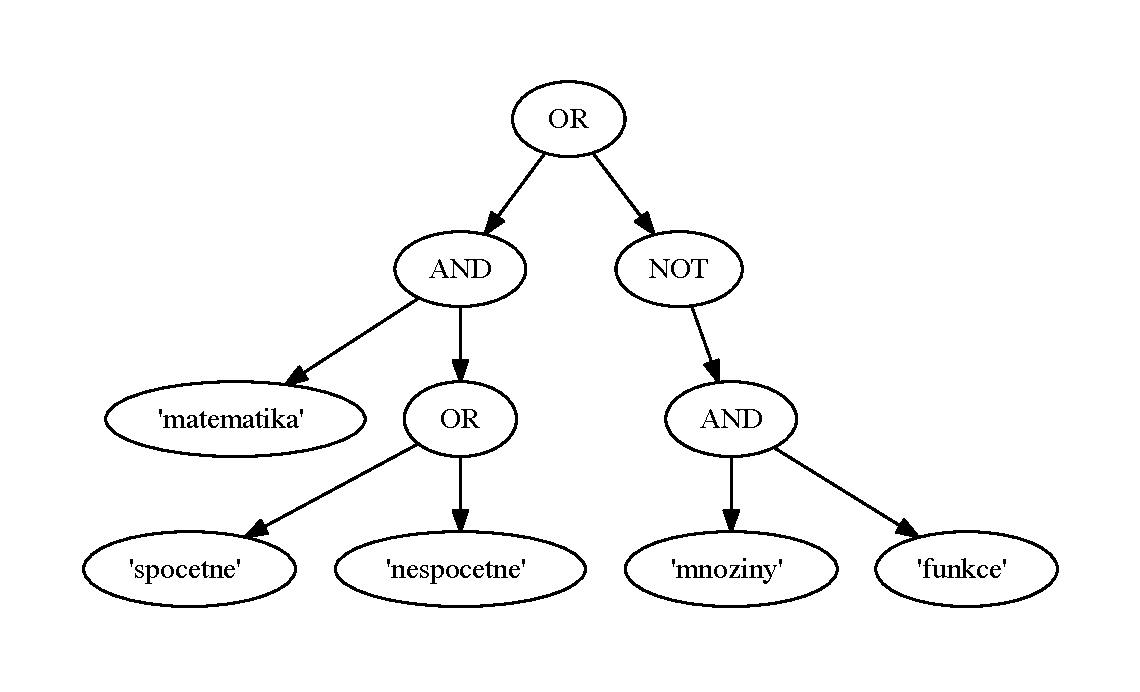
\includegraphics[width=14cm]{obrazky/syntactic_tree.pdf}
  \caption{Syntaktický strom}
  \label{fig:syntree}
\end{figure}

Nakonec celý výraz zjednodušíme -- odstraníme uzly, které obsahují stop slova, protože stop slova nepoužíváme při vyhledávání a převedeme slova na stemy. 

\sssection{Vyhledání odpovídajících dokumentů}

Ve chvíli, kdy máme syntaktický strom, se můžeme pustit do hledání dokumentů. K tomu využijeme vybudovaný index, který nám umožňuje snadno zjistit, v jakých dokumentech se vyskytuje dané slovo. Pro účely popisu mechanismu si definujeme funkci $\getdocs$, která bere na vstupu dotaz (syntaktický strom) $Q$ a na výstupu vrací množinu dokumentů, které odpovídají zadanému dotazu. Tato funkce se bude chovat odlišně v závislosti na tom, jak vypadá dotaz $Q$. 

Dále označme $\alldoc$ množinu všech dokumentů a $\alpha$ a $\beta$ nechť označují nějaké dotazy. 

\begin{itemize}
\item Je-li $Q=s$, kde $s$ je nějaký stem, pak funkce $\getdocs$ vrátí množinu dokumentů, které obsahují daný stem, což vyčteme z indexu. Formálně to můžeme zapsat jako:
$$
\getdocs_s = \left\{d\in \alldoc\sep s\in d\right\}.
$$
\item Je-li dotaz ve tvaru Q = \uv{$\alpha$ AND $\beta$}, pak $\getdocs_Q = \getdocs_\alpha \cap \getdocs_\beta$.
\item Je-li dotaz ve tvaru Q = \uv{$\alpha$ OR $\beta$}, pak $\getdocs_Q = \getdocs_\alpha \cup \getdocs_\beta$.
\item Je-li dotaz ve tvaru Q = \uv{NOT $\alpha$}, pak $\getdocs_Q = \alldoc\setminus\getdocs_\alpha$.
\end{itemize}

Postupnou aplikací těchto pravidel dostaneme množinu výsledných dokumentů $R$. V dalším kroku tyto dokumenty seřadíme podle relevance. 

\sssection{Seřazení dokumentů}

V současné chvíli máme množinu dokumentů $\getdocs_Q$. Aby byl vyhledávač smysluplný, měl by tyto dokumenty seřadit podle toho, jak relevantní dané dokumenty vzhledem k položenému dotazu jsou. To je obecně nelehký úkol. Ve vyhledávači je pak použit standardní $\tfidf$ algoritmus popsaný v části \ref{tfidf}

Abychom mohli ohodnotit jednotlivé dokumenty, potřebujeme znát slova, vůči kterým máme dokumenty ohodnocovat. Odstraníme tak z dotazu všechny operátory a dostaneme množinu všech slov $S$. Vůči těmto slovům budeme dokumenty hodnotit. 

K tomu už využijeme $\tfidf$ algoritmus -- pro každé slovo z množiny $S$ a pro každý dokument z množiny $\getdocs_Q$ spočítáme jeho $\tfidf$ skóre; poté tato skóre sečteme a dokumenty seřadíme sestupně podle tohoto skóre. Skóre $\score_{d,S}$ dokumentu $d$ tak udává vzorec:
$$\score_{d,S}=\sum_{s\in S} \tfidf_{s, d}.$$

Toto základní skóre ještě dále upravíme podle toho, zda se klíčová slova z dotazu nevyskytují v důležitých částech dokumentu, konkrétně jde o název, adresa a popisek stránky. Za každé klíčové slovo, které se vyskytuje v názvu stránky $d$ nebo v adrese stránky, ztrojnásobíme hodnotu $\score_{d,S}$. Za každé klíčové slovo, které se vyskytuje v popisu stránky $d$, zdvojnásobíme hodnotu $\score_{d,S}$. Ve výsledku tak dostáváme funkci $\rank$, která nejprve vypočte hodnotu $\score_{d,S}$ a poté aplikuje pravidla o ztrojnásobení a zdvojnásobení. Funkce $\rank$ bere na vstupu dva parametry: dokument $d$, pro který počítáme skóre a slova $S$ z dotazu $Q$.

\begin{figure}
\begin{algorithmic}
\Function{rank}{$d, S$}
    \State $score \gets \score_{d, S}$
    \ForAll{$s \in S$} 
    	\If{$s \in \mbox{title}(d) \quad\vee\quad s \in \mbox{url}(d)$}
    		\State $score \gets score \cdot 3$
    	\EndIf
    	\If{$s \in \mbox{description}(d)$}
    		\State $score \gets score \cdot 2$
    	\EndIf
    \EndFor
    \State \Return $score$
\EndFunction
\end{algorithmic}
\end{figure}



Nyní seřadíme dokumenty $\getdocs_Q$ do $n$-tice $\addh{d_1, d_2, \ldots, d_n}$, kde 
$$n=\left|\getdocs_Q\right|\quad\mbox{a}\quad \bigcup_{i=1}^n d_i=\getdocs_Q$$ 
tak, aby platilo $\rank_{d_1, S} \ge \rank_{d_2, S} \ge \ldots \ge \rank_{d_n, S}$.

Tato seřazená $n$-tice je výstupem algoritmu vyhledávání. 





%%%%%%%%%%%%%%%%%%%%%%%%%%%%%%%%%%%%%%%%%%%%%%%%%%%%%%%%%%%%%%
%%%%%%%%%%%%%%%%%%%% FCA ČÁST VYHLEDÁVAČE %%%%%%%%%%%%%%%%%%%%
%%%%%%%%%%%%%%%%%%%%%%%%%%%%%%%%%%%%%%%%%%%%%%%%%%%%%%%%%%%%%%

\newpage
\section{Hledání souvisejících dokumentů}
V této kapitole bude popsána druhá část vyhledávače, která se stará o nalezení souvisejících dotazů. 

\ssection{O co nám půjde}

\sssection{Motivace}

Pokud uživatel položí vyhledávači nějaký dotaz, vyhledávač odpoví nějakým seznamem dokumentů, které jsou podle něj nejvíce relevantní. Pokud má uživatel štěstí, bude v tomto seznamu dokument, který zrovna potřebuje najít. Pokud bude mít velké štěstí, pak bude tento dokument na předních místech v seznamu. 

Pokud ale toto štěstí mít nebude a dokument se mu nepodaří nalézt, musí uživatel nějakým způsobem přeformulovat svůj dotaz tak, aby vyhledávač vrátil jinou sadu výsledků. Obecně může upravit dotaz třemi různými způsoby. Může

\begin{enumerate}
\item přidat k dotazu jedno či více slov, díky čehož obdrží méně výsledků,
\item změnit jedno či více slov, díky čehož obdrží podobné výsledky,
\item odebrat jedno či více slov, díky čehož obdrží více výsledků.
\end{enumerate}

V různých situacích se hodí různé postupy. Pokud jsme zadali příliš konkrétní dotaz, na který vyhledávač odpověděl málo dokumenty, bude vhodné odebrat některá klíčová slova dotazu, abychom získali více výsledků. Pokud jsme naopak zadali příliš obecný dotaz, můžeme přidat nějaká klíčová slova, abychom obrželi méně dokumentů, která ale lépe odpovídají na náš dotaz. 

\sssection{Hlavní cíl}

Hlavním cílem vyhledávače je nacházet zmíněné úpravy dotazu automaticky. Tyto úpravy můžeme hledat například pomocí historie dotazů, pokud danou historii máme. Pokud uživatel položí dotaz \uv{hosting php}, můžeme se podívat do historie vyhledávání a nalézt všechny dotazy, které obsahují alespoň jedno ze slov v dotazu a z této množiny dotazů pak můžeme nějakým postupem vybrat související dotazy pro všechny tři kategorie úprav. Můžeme například zjistit, že z konkrétnějších dotazů je nejvíce hledaný dotaz \uv{hosting php mysql}, z podobných \uv{server php} a podobně. 

My ale použijeme jiný postup. Všechny související dotazy budeme hledat pouze na základě znalostí sady dokumentů. Nebudeme k tomu využívat žádné dodatečné informace, všechno si spočítáme pouze ze samotných dokumentů.

K tomu využijeme formální konceptuální analýzu, která v daných datech vyhledává jisté shluky potenciálně zajímavých dat a zároveň je ukládá do hierarchie, se kterou můžeme dále pracovat. Pro základní představu si můžeme představit výstup FCA jako Hasseův diagram, kde jeden z uzlů -- ten musíme nějak najít -- představuje aktuální výsledky, které nám vyhledávač zobrazil, \uv{otcové} tohoto uzlu jsou obecnější dotazy, \uv{synové} jsou konkrétnější dotazy a \uv{sourozenci} jsou podobné dotazy. 

\sssection{Výstup vyhledávače}

Jak by měl vypadat výstup vyhledávače? Vyhledávač by měl zobrazit seřazenou sadu klasických výsledků, na tom se nic nemění. Dále by měl spočítat návrhy na úpravu dotazů ve všech třech kategorií -- konkrétnější, podobný a obecnější dotaz. Pokud tyto návrhy existují, což není vždy, měl by je uživateli zobazit. Tyto návrhy by měl vyhledávač opět seřadit podle relevance, tj. aby první úpravy dotazů byly nejsmysluplnější. Výstup pro dotaz \uv{příležitostné příjmy} by měl vypadat přibližně takto:

\begin{verbatim}
1. Příležitostná činnost
2. Ostatní příjmy a daňové přiznání
3. ...

+ sleva | + potvrzení
+/- sleva, příjmy | +/- příjmy, paušální
- příležitostné | -příjmy
\end{verbatim}

Nejprve máme klasický seznam dokumentů setříděných podle relevance. Následující tři řádky jsou hlavním výsledkem vyhledávače, jsou to návrhy, jak upravit dotaz. 

Na prvním řádku jsou klíčová slova, která můžeme k dotazu přidat. Tj. první návrh, \code{+sleva}, nám říká, abychom zkusili vyhledat dotaz \uv{příležitostné příjmy sleva}, čímž bychom měli získat dokumenty, které nám řeknou, zda můžeme u příležitostných příjmů uplatnit nějakou slevu. To zní jako smysluplný dotaz. 

Na druhém řádku máme podobné dotazy. Nabízí nám to vyhledat \uv{sleva příjmy}, čímž bychom měli dostat dokumenty, které se věnují celkově slevám, které můžeme během danění příjmů uplatnit. Druhým dotazem, \uv{paušální příjmy}, bychom se měli dostat k informacím o paušálních výdajích, které můžeme uplatnit při danění příjmů. 

Na poslední, řádku nám vyhledávač nabízí odstranit slova, abychom získali více dokumentů. 

\ssection{Teoretické základy formální konceptuální analýzy}
\sssection{Neformální úvod}
Formální konceptuální analýza (dále jen FCA) pracuje s tabulkovými daty. V řádcích máme objekty, ve sloupcích máme atributy objektů. Obsahem každé buňky je pak informace, zda daný objekt má daný atribut. Tato informace je binární, daný objekt buď daný atribut má, nebo nemá. 

V tabulce \ref{tab.con1} je příklad takových tabulkových dat. V řádcích jsou objekty -- živočichové či rostliny. Ve sloupcích pak jsou jednotlivé atributy, což jsou nějaké vlastnosti, které dané objekty mohou mít. Pod tabulkou je legenda k jednotlivým atributům. Například první atribut $a$ je \uv{potřebuje k životu vodu}. Každý živočich a každá rostlina potřebuje k životu vodu, takže v celém sloupečku je křížek. Druhý atribut $b$ je \uv{žije ve vodě}. Zde už není křížek všude, takový pes ve vodě nežije. 


\begin{table}
\begin{center}
\begin{tabular}{r|ccccccccc}
\toprule
&a&b&c&d&e&f&g&h&i\\
\midrule
Pijavice&\yes&\yes&&&&&\yes\\
Cejn&\yes&\yes&&&&&\yes&\yes\\
Žába&\yes&\yes&\yes&&&&\yes&\yes\\
Pes&\yes&&\yes&&&&\yes&\yes&\yes\\
Bodlák&\yes&\yes&&\yes&&\yes\\
Rákosí&\yes&\yes&\yes&\yes&&\yes\\
Fazole&\yes&&\yes&\yes&\yes\\
Kukuřice&\yes&&\yes&\yes&&\yes\\
\bottomrule
\end{tabular}
\end{center}
\caption{Formální kontext} \label{tab.con1}

\begin{center}
$a$: potřebuje k životu vodu, $b$: žije ve vodě, $c$: žije na zemi,\\ $d$: potřebuje chlorofyl, $e$: dvouděložná rostlina, $f$: jednoděložná rostlina,\\ $g$: může se pohybovat, $h$: má končetiny, $i$: kojí potomky
\end{center}
\end{table}


Takové tabulce s daty říkáme \strong{kontext}. V tomto kontextu pak hledáme shluky potenciálně zajímavých dat. Shlukem může být například množina $\adds{\mbox{Cejn, Žába, Pes}}$, protože všechna tato zvířata sdílí společné atributy $\adds{a, g, h}$ -- potřebují vodu k životu, mohou se pohybovat a mají končetiny. Zároveň platí, že cejn, žába a pes žádné další společné atributy nesdílí a podobně u atributů: žádný další objekt už nemá právě tyto tři společné vlastnosti. Takové dvě množiny objektů a atributů pak tvoří \strong{koncept}. Množinu objektů konceptu nazýváme \strong{extent} a množinu atributů \strong{intent}. 

Když se podíváme na tabulku, zjistíme, že koncept je tvořený křížky, které dohromady tvoří \uv{rozházený obdélník}. Pokud bychom ale sloupce, které reprezentují množinu společných atributů, přesunuly k sobě, získali bychom hezký obdélník (v tomto případě dokonce čtverec). Koncept je zvýrazněný v tabulce \ref{tab.con2} Vždy nás zajímá maximální obdélník, tj. pokud existuje objekt nebo atribut, který můžeme přidat a opět získáme obdélník, přidáme ho. 

\begin{table}
\begin{center}
\begin{tabular}{r|ccccccccc}
\toprule
&b&c&d&e&f&g&h&a&i\\
\midrule
Pijavice&\yes&&&&&\yes&&\yes\\
Cejn&\yes&&&&&\fyes&\fyes&\fyes\\
Žába&\yes&\yes&&&&\fyes&\fyes&\fyes\\
Pes&&\yes&&&&\fyes&\fyes&\fyes&\yes\\
Bodlák&\yes&&\yes&&\yes&&&\yes\\
Rákosí&\yes&\yes&\yes&&\yes&&&\yes\\
Fazole&&\yes&\yes&\yes&&&&\yes\\
Kukuřice&&\yes&\yes&&\yes&&&\yes\\
\bottomrule
\end{tabular}
\end{center}
\caption{Formální kontext se zvýrazněným konceptem} \label{tab.con2}
\end{table}


To samozřejmě není jediný koncept, který kontext obsahuje. Ve skutečnosti tento kontext obsahuje 19 konceptů. Zkusíme si najít další. Existuje něco, co žije na zemi i ve vodě? Hledáme tak objekty, které mají atributy $\adds{b, c}$. Pohledem do tabulky zjistíme, že tyto vlastnosti má žába a rákosí. Nicméně ještě jsme nenalezli koncept, protože nevíme, jestli náhodou tyto objekty nesdílí ještě nějaký další atribut. Vzhledem k tomu, že všechny objekty mají atribut $a$, musíme ho přidat do množiny atributů. Tím už získáme koncept s objekty $\adds{\mbox{žába, rákosí}}$ a atributy $\adds{a, b, c}$.

Řekli jsme, že formální konceptuální analýza zároveň řeší i hierarchii shluků. Ta se řeší pomocí relace inkluze. Můžeme říci, že koncept, který se skládá z extentu $\adds{\mbox{pojavice, cejn, žába a pes}}$ a intentu $\adds{a, g}$ je obecnější než koncept $\adds{\mbox{cejn, žába a pes}}$ a $\adds{a, g, h}$. 

První koncept můžeme pojmenovat \uv{pohybující se živočichové}, druhý koncept by byl \uv{živočichové, kteří k pohybu využívají končetiny}. Druhý koncept obsahuje všechny atributy jako první koncept, plus jeden navíc -- ten nějakým způsobem konkretizuje tento koncept. U objektů to platí naopak. Druhý koncept má více atributů, ale méně objektů. To je logické, pokud zvýšíme počet atributů, které objekty musí mít, zvýšíme tím na objekty nároky a objektů ubyde. 

\sssection{Formální definice FCA}

\begin{mydef}[Formální kontext]
Formální kontext je trojice $\addsp{X, Y, I}$, kde $X$ je neprázdná množina objektů, $Y$ je neprázdná množina atributů a $I$ je binární relace mezi $X$ a $Y$, tj. $I\subseteq X\times X$.
\end{mydef}

V předchozím příkladě byla množina $X$ rovna programům a množina $Y$ byla rovna vlastnostem programů. Relace $I$ pak vyznačuje, zda má objekt $x$ atribut $y$. Objekt $x$ má atribut $y$ právě tehdy když $\addsp{x, y}\in I$. Formální kontext, jak jsme viděli, může být reprezentován pomocí tabulky. 

\begin{mydef}[Šipečkové operátory]
Pro kontext $\context$ definujeme operátory $\up:2^X\rightarrow2^Y$ a $\down:2^Y\rightarrow2^X$, tak že pro každé $A\subseteq X$ a $B\subseteq Y$:
\begin{eqnarray}
A\up&=&\adds{y\in Y\sep \foreach x \in A: \addsp{x, y}\in I}\\
B\down&=&\adds{x\in X\sep\foreach y\in B:\addsp{x, y} \in I}
\end{eqnarray}
\end{mydef}

Tyto operátory umožňují zjistit společné vlastnosti. Operátor $\up$ nám zjistí všechny atributy, které mají všechny objekty v $A$ společné. Operátor $\down$ nám zjistí všechny objekty, které sdílí všechny atributy z $B$. 

Pokud se vrátíme ke kontextu v tabulce \ref{tab.con1}, tak:

\begin{eqnarray*}
\adds{\mbox{Xcode}}\up&=&\adds{\mbox{Debug, Barvy}}\\
\adds{\mbox{PSPad, Smultron}}\up&=&\adds{\mbox{Start, Barvy}}\\
\adds{\mbox{TextEdit, Poznámkový Blok}}\up&=&\adds{\mbox{Start, Výchozí}}\\
A\up&=&\emptyset\\
\adds{\mbox{Multi, Java}}\down&=&\adds{\mbox{Aptana, NetBeans}}\\
\adds{\mbox{Debug, Výchozí}}\down&=&\emptyset\\
\adds{\mbox{Barvy, Start}}\down&=&\adds{\mbox{PSPad, Smultron}}
\end{eqnarray*}

\begin{mydef}[Formální koncept]
Formální koncept v kontextu $\context$ je dvojice $\AB$, $A\subseteq X$, $B\subseteq Y$ tak, že:
$$A\up=B\logand B\down =A.$$

Množině $A$ říkáme \uv{extent} a množině $B$ \uv{intent}.
\end{mydef}

Takto definovaný formální koncept odpovídá naší předchozí představě o konceptu. Pokud jsme měli danou množinu objektů, pak jsme našli sdílené atributy. K těmto sdíleným atributům jsme následně nalezli objekty, které všechny tyto atributy sdílí, což mohlo být více objektů, než jaké jsme měli na začátku. Ve chvíli, kdy se k těmto objektům pokusíme najít sdílené atributy, nenalezneme již žádný nový.

V tabulce \ref{tab.con1} tak můžeme najít například koncept 
$$\adds{\adds{\mbox{PSPad, Smultron}}, \adds{\mbox{Barvy, Start}}},$$ 
protože 
$$\adds{\mbox{PSPad, Smultron}}\up=\adds{\mbox{Barvy, Start}} \logand \adds{\mbox{Barvy, Start}}\down=\adds{\mbox{PSPad, Smultron}}.$$


\begin{mydef}[Uspořádání konceptů]
\label{def.order}
O konceptech $\addsp{A_1, B_1}, \addsp{A_2, B_2}$ kontextu $\context$ řekeneme, že
$$\addsp{A_1, B_1}\le\addsp{A_2, B_2}\quad\pravekdyz\quad A_1\subseteq A_2 \quad(B_2\subseteq B_1).$$
\end{mydef}

Relaci menší nebo rovno mezi koncepty můžeme interpretovat jako relaci \uv{být konkrétnější koncept}. Pokud pro koncepty platí $\addsp{A_1, B_1}\le\addsp{A_2, B_2}$, pak koncept $\addsp{A_1, B_1}$ je konkrétnější než koncept $\addsp{A_2, B_2}$. 

\begin{mydef}[Konceptuální svaz]
Pro kontext $\context$ definujeme množinu všech formálních konceptů $\lattice$ z $\context$. Tedy
$$\lattice=\adds{\addsp{A, B}\in 2^X\times 2^Y\sep A\up=B\logand B\down=A}.$$

Dvojice $\addsp{\lattice, \le}$ pak představuje konceptuální svaz. 
\end{mydef}

\begin{mydef}[Nejmenší extent obsahující $A$]
Nejmenší extent, který obsahuje množinu $A$, je extent $A\updown$. Nejmenší intent, který obsahuje množinu $B$, je intent $B\downup$. 
\end{mydef}

\begin{mydef}[Hlavní věta konceptuálních svazů]

\end{mydef}

%%% Závěr práce v~češtině
\begin{conclusions-cz}
  Závěr práce v češtině.
\end{conclusions-cz}


%%% Závěr práce v~angličtině
\begin{conclusions-en}
  Conclusion in english.
\end{conclusions-en}


\end{document}
